\documentclass[11pt]{article}

\usepackage{extras} % Se extras.sty

\begin{document}
\begin{titlepage}
\begin{center}

{\Large\bfseries TSEA56 - Kandidatprojekt i elektronik \\ LIPS Teknisk dokumentation}

\vspace{5em}

Version 1.0

\vspace{5em}
Grupp 4 \\
\begin{tabular}{rl}
Hynén Ulfsjöö, Olle&\verb+ollul666+
\\
Wasteson, Emil&\verb+emiwa068+
\\
Tronje, Elena&\verb+eletr654+
\\
Gustafsson, Lovisa&\verb+lovgu777+
\\
Inge, Zimon&\verb+zimin415+
\\
Strömberg, Isak&\verb+isast763+
\\
\end{tabular}

\vspace{5em}
\today

\vspace{16em}
Status
\begin{longtable}{|l|l|l|} \hline

Granskad & - & - \\ \hline
Godkänd & - & - \\ \hline
 
\end{longtable}

\end{center}
\end{titlepage}

\pagebreak
\begin{center}

\section*{PROJEKTIDENTITET}
2016/VT, Undsättningsrobot Gr. 4

Linköpings tekniska högskola, ISY
\vspace{5em}
%\begin{center}

\begin{tabular}{|l|l|l|l|} \hline
\textbf{Namn} & \textbf{Ansvar} & \textbf{Telefon} & \textbf{E-post}  \\ \hline 
Isak Strömberg (IS) & Projektledare & 073-980 38 50 & isast763@student.liu.se \\ \hline
Olle Hynén Ulfsjöö (OHU)& Dokumentansvarig & 070-072 91 84 & ollul666@student.liu.se \\ \hline
Emil Wasteson (EW) & Hårdvaruansvarig & 076-836 61 66 & emiwa068@student.liu.se \\ \hline
Elena Tronje (ET) & Mjukvaruansvarig & 072-276 92 93 & eletr654@student.liu.se \\ \hline
Zimon Inge (ZI)& Testansvarig & 070-171 35 18 & zimin415@student.liu.se \\ \hline
Lovisa Gustafsson (LG) & Leveransansvarig & 070-210 32 53 & lovgu777@student.liu.se \\ \hline
\end{tabular}

%\end{center}

E-postlista för hela gruppen: isast763@student.liu.se

\vspace{5em}
Kund: ISY, Linköpings universitet 
tel: 013-28 10 00, fax: 013-13 92 82 \\
Kontaktperson hos kund: Mattias Krysander \\
tel: 013-28 21 98, e-post: matkr@isy.liu.se \\

\vspace{5em}
Kursansvarig:  Tomas Svensson\\
tel: 013-28 13 68, e-post: tomass@isy.liu.se \\
Handledare: Peter Johansson \\
tel: 013-28 13 45, e-post: peter.a.johansson@liu.se
\end{center}
\pagebreak

\tableofcontents

\pagebreak

\section*{Dokumenthistorik}
\begin{table}[h]
\begin{tabular}{|l|l|l|l|l|} \hline

\textbf{Version} & \textbf{Datum} & \textbf{Utförda förändringar} & \textbf{Utförda av} & \textbf{Granskad} \\ \hline
1.0 & - &  Första utkastet & Grupp 4 & - \\ \hline
\end{tabular}
\end{table}

\pagebreak
\pagenumbering{arabic}

\begin{flushleft}
\section{Inledning}
\textit{Bakgrund och syfte}

Projektets syfte är att konstruera en undsättningsrobot med kartläggning. Detta dokument syftar till att ge en detaljerad teknisk beskrivning av projektet på en nivå där resultatet ska kunna återskapas. Innehållet består av detaljerade beskrivningar av systemets olika delar, dess mjuk- och hårdvarukomponenter samt implementationen av dessa.

\section{Produkten}
\textit{En bild på produkten och en beskrivning av hur den fungerar. Beskriv vad den används till.}

Produkten som konstruerats är en undsättningsrobot. Den består av ett chassi med fyra hjul, ett batteri, en av/på-brytare samt en gripklo. På chassit är huvudmodulen, sensormodulen och styrmodulen ihopkopplade via en I\textsuperscript{2}C-buss för kommunikation dem emellan. Roboten kommunicerar med datormodulen via Bluetooth\textsuperscript{\circledR}. En övergripande bild av produkten återfinns i figur \ref{overview}. Gripklon kontrolleras av styrmodulen och sensormodulen tar in data från sensorerna. För att fästa sensorerna på chassit används 3D-printade fästen.

Varje modul har en processor samt annan nödvändig hårdvara, som lågpassfilter och brytare, kopplade på ett virkort. Virkorten kan användas som grund för att tillverka kretskort med motsvarande funktion. 

Robotens uppgift är att söka av en labyrint bestående av 40 cm breda korridorer med hjälp av en avsökningsalgoritm och identifiera en nödställd som sänder ut IR-ljus. När målet är identifierat ska kortaste vägen mellan labyrintens ingång och målet bestämmas. Efter det ska roboten hämta en förnödenhet vid starten, köra kortaste vägen till den nödställda och lämna av förnödenheten för att sedan ta sig tillbaka samma väg till starten. Roboten kartlägger labyrinten internt under tiden den utforskar den och lagrar informationen för att kunna skicka den till datormodulen för uppritning. 


\begin{figure}[!htbp]
\centering
\noindent\resizebox{\linewidth}{!}{
	\documentclass{minimal}
\usepackage{tikz}
%\usetikzlibrary{calc,trees,positioning,arrows,chains,shapes.geometric,decorations.pathreplacing,decorations.pathmorphing,shapes,matrix,shapes.symbols}
\usetikzlibrary{positioning}
\usetikzlibrary{shapes}

\begin{document}
\begin{center}
\begin{tikzpicture}[scale=1]
\tikzset{every node/.style={inner sep=10pt, minimum width=3 cm}}
%\draw[help lines,step=5mm,gray!20] (-5,-10) grid (5,0);
\node[draw, fill=white] (Huvudmodul)  {\textbf{Huvudmodul}};
\node[draw,below left= of Huvudmodul] (Sensormodul) {\textbf{Sensormodul}};
\node[draw,below right = of Huvudmodul] (Styrenhet) {\textbf{Styrenhet}};
\node[draw, above = of Huvudmodul] (Datormodul) {\textbf{Datormodul}};
\node[ellipse,draw, right = of Datormodul] (Användare) {\textbf{Användare}};

\draw[->] (Huvudmodul) [out=300, in= 90] to (Styrenhet);
\draw[->] (Sensormodul) [out=90, in=240] to (Huvudmodul);
\draw[<->] (Huvudmodul) to (Datormodul);
\draw[<->] (Datormodul) to (Användare);
\end{tikzpicture}
\end{center}

\vspace{10em}

\begin{center}
\begin{tikzpicture}[scale=1]
\tikzset{every node/.style={inner sep=10pt, minimum width=3 cm}}
%\draw[help lines,step=5mm,gray!20] (-5,-10) grid (5,0);

\node[draw] (Sensormodul) {\textbf{Sensormodul}};
\node[above right = of Sensormodul,minimum width=0,inner sep=2pt] (Huvudmodul) {Huvudmodul};

\node[below left = of Sensormodul, minimum width = 0, inner sep = 2pt] (Sensor) {Sensorer};


\draw[->] (Sensor) [out=0,in=270] to node [sloped, midway, below] {spänningsnivåer} (Sensormodul);
\draw[->] (Sensormodul) [out=90,in=180] to node [sloped,midway, above] {enheter}  (Huvudmodul);

\end{tikzpicture}
\end{center}

\vspace{10em}

\begin{center}
\begin{tikzpicture}[scale=1]
\tikzset{every node/.style={inner sep=10pt, minimum width=3 cm}}
%\draw[help lines,step=5mm,gray!20] (-5,-10) grid (5,0);

\node[draw] (Styrmodul) {\textbf{Styrmodul}};
\node[above left = of Styrmodul,minimum width=0,inner sep=2pt] (Huvudmodul) {Huvudmodul};

\node[below right = of Styrmodul, minimum width = 0, inner sep = 2pt] (Motorer) {Motorer};
%\node[below left = of Styrmodul, minimum width = 0, inner sep= 2pt] (Gripklo) {Gripklo}


\draw[->] (Styrmodul) [out=270,in=180] to node [sloped, midway, below] {spänningsnivåer} (Motorer);
\draw[<-] (Sensormodul) [out=90,in=0] to node [sloped,midway, above] {kommandon}  (Huvudmodul);

\end{tikzpicture}
\end{center}

\vspace{10em}

\begin{center}
\begin{tikzpicture}[scale=1]
\tikzset{every node/.style={inner sep=10pt, minimum width=3 cm}}
%\draw[help lines,step=5mm,gray!20] (-5,-10) grid (5,0);

\node[draw] (Datormodul) {\textbf{Datormodul}};
\node[below = 10 em of Datormodul,minimum width=0,inner sep=2pt] (Huvudmodul) {Huvudmodul};
\node[right = of Datormodul, ellipse, draw] (Användare) {Användare};

%\node[below right = of Styrmodul, minimum width = 0, inner sep = 2pt] (Motorer) {Motorer};
%\node[below left = of Styrmodul, minimum width = 0, inner sep= 2pt] (Gripklo) {Gripklo}


\draw[->] (Datormodul) [out=30,in=150] to node [midway, above] {karta} (Användare);
\draw[<-] (Datormodul) [out=-30,in=210] to node [midway, below] {kommandon}  (Användare);

\draw[->] (Datormodul) [out=300,in=60] to node [near end, right] {kommandon} (Huvudmodul);
\draw[<-] (Datormodul) [out=240,in=120] to node [near end, left] {sensordata} (Huvudmodul);

\end{tikzpicture}
\end{center}


\end{document}}
	\caption{Det totala systemet \label{overview}}	
\end{figure}

\pagebreak


\section{Teori}
Nedan följer en sammanfattning av den teori som robotens reglering och optimering bygger på.

\subsection{Optimering}


\subsection{Reglering}
\label{subsection:reglering}
\section{Systemet}
\textit{Ett översiktligt blockschema och en beskrivning av hela systemet.}

Roboten i sin miljö finns illustrerad i figur \ref{system}. Den kan både köras manuellt och autonomt, något som bestäms av en brytare på roboten. Kommunikationen med datormodulen är dubbelriktad via Bluetooth\textsuperscript{\circledR}. Roboten ska klara sitt uppdrag utan kommunikation med datormodulen, det vill säga att kartläggning, styrning och optimering av kortaste väg sker lokalt hos roboten. Banan är uppbyggd enligt banspecifikationen och uppdraget utförs enligt tävlingsreglerna, se appendix [??].

\begin{figure}[htbp]
\centering
\noindent\resizebox{.8\linewidth}{!}{
	\input{images/bana}}
	\caption{Översikt av banan\label{system}}	
\end{figure}

\subsection{Beskrivning av systemet}
Roboten navigerar med hjälp värden som fås av sensormodulens sensorer. En lasersensor, fäst på ett servo, mäter avstånd framåt, fyra IR-sensorer mäter robotens avstånd till sidoväggarna, ett gyroskop mäter robotens vinkelhastighet och en IR-detektor identifierar den nödställde. Med jämnna intervall kommunicerar sensormodulen dessa värden till huvudmodulen, som i sin tur vidarebefordrar de till styrmodulen. 

I styrmodulen är en regleringsmodell implementerad, vilken säkerställer att roboten färdas i mitten av korridorerna samt kan rotera både 90 och 180 grader utan att stöta mot väggar. Önskade värden kan skrivas ut på en LCD-display, vilken också är en del av styrmodulen.

Under färden sker autonomt kartläggning och beräkning av kortaste väg mellan ingången och den nödställde. När roboten är uppkopplad mot datormodulen ritar mjukvaran på datorn successivt upp en karta och presenterar utvalda mätvärden i realtid. 

När den kortaste vägen är funnen använder roboten denna rutt för att förse den nödställde med en förnödenhet. Förnödenheten transporteras med hjälp av robotens gripklo, som kontrolleras av styrmodulen.

På systemnivå är det om målet är funnet och om kortaste väg kan garanterats som avgör robotens beslut, vilket figur \ref{blockSystem} illustrerar.

\begin{figure}[htbp]
\centering
\noindent\resizebox{1\linewidth}{!}{
	\documentclass[border=10px]{standalone}
\usepackage{tikz}
\usetikzlibrary{patterns}
\usetikzlibrary{shapes.geometric}
\usetikzlibrary{shapes.arrows}
\usepackage{amssymb}
\usetikzlibrary{calc}
\usepackage{verbatim}

\pagestyle{empty}
\begin{document}

\tikzstyle{decision} = [diamond, draw,
    text width=4em, text badly centered, node distance=3cm, inner sep=0pt]
    
\tikzstyle{block} = [rectangle, draw,
    text width=5em, text centered, rounded corners, minimum height=4em]
	
\begin{tikzpicture}[scale=1]

%http://www.texample.net/tikz/examples/simple-flow-chart/

\node[block](start){Start};
\node[decision, below of = start, aspect = 2, text width = 8 em] (foundTarget) {Målet funnet?};
\node[block, below of = foundTarget, node distance = 3cm, text width = 7em] (explore) {Utforska enligt högerföljning};
\node[decision, right of = foundTarget, text width = 6em, aspect = 2, node distance = 6cm] (foundShortestPath) {Garanterat funnit kortaste väg?};
\node[block, below of = foundShortestPath, node distance = 3cm, text width = 7em] (exploreTargetFound) {Utforska enligt högerföljning och optimering};
\node[block, right of = foundShortestPath, node distance = 5cm] (pickUp) {Hämta förnödenhet vid start};
\node[block, right of = pickUp, node distance = 3cm, text width = 6em] (shortestPath) {Från start följ kortaste väg till målet};
\node[block, right of = shortestPath, node distance = 3cm] (drop) {Lämna förnödenhet};
\node[block, below of = drop, node distance = 3cm, text width = 7em] (return) {Återvänd till startpunkt den kortaste vägen};
\node[block, below of = return, node distance = 3cm] (stop) {Slut};

\draw[->](start) --  (foundTarget);
\draw[->](foundTarget) -- node[near start, right]{nej} (explore);
\draw[->] (explore.west) -| ++(-1,3) -| (foundTarget.west);
\draw[->](foundTarget) -- coordinate[midway] (aux) node[near start, above]{ja} (foundShortestPath);
\draw[->] (foundShortestPath) -- node[near start, right]{nej}(exploreTargetFound);
\draw[->] (exploreTargetFound) -| (aux);
\draw[->] (foundShortestPath) -- node[near start, above]{ja}(pickUp);
\draw[->] (pickUp) -- (shortestPath);
\draw[->] (shortestPath) -- (drop);
\draw[->] (drop) -- (return);
\draw[->] (return) -- (stop);

	\end{tikzpicture}
	
\end{document}}
	\caption{Övergripande blockschema för systemet}	\label{blockSystem}
\end{figure}

\section{Begränsningar} 
Roboten är begränsad till att navigera i korridorer som är ca 40 cm breda och klarar enbart av korsningar med 90 gradersvinklar.

\section{Modulerna}
\textit{Innehåller mera detaljerade blockschemor och beskrivningar av varje modul. Tänk på läsbarheten och växla mellan figurer och text.}
I detta avsnitt följer en detaljerad beskrivning av systemets ingående moduler. 

\subsection{Huvudmodulen}
Huvudmodulen har som uppgift att ta emot och förmedla information mellan de andra modulera, hantera den interna kartläggnigen samt att ta alla övergripande beslut. Bluetooth\textsuperscript{\circledR} används för att kommunicera med datormodulen och en avbrottsstyrd I\textsuperscript{2}C-buss används för att kommunicera med sensor- och styrmodulen, vilket visas i figur \ref{communication}. När det kommer till prioriteringen av sensor- och styrmodul har styrmodulen kopplats till en extern avbrottsingång med högre prioritet än sensormodulen.

\begin{figure}[htbp]
\noindent\resizebox{.97\textwidth}{!}{
	\documentclass[border=20pt]{standalone}
\usepackage{tikz}
\usetikzlibrary{positioning}
\usetikzlibrary{calc}
\usetikzlibrary{decorations.pathmorphing}
\usepackage{amssymb}
\usetikzlibrary{shapes,arrows}

\begin{document}
	\begin{tikzpicture}[scale=1]
		
		\tikzset{every node/.style={thick, draw=black, align=center, minimum height=40pt, text width=100pt, minimum width=100pt}}
		\node(datormodul) {Datormodul};
		\node[right=10pt of datormodul,minimum height=20pt, minimum width=10pt,text width=10pt] (bt1) {\includegraphics{bluetooth}};
		
		\node[right=40pt of bt1,minimum height=20pt, minimum width=10pt,text width=10pt] (bt2) {\includegraphics{bluetooth}};
		
		\node[right=10pt of bt2] 			(huvudmodul) 	{Huvudmodul};
		\node[below=-10pt of huvudmodul,draw=none] (master) {\textit{master}};
		\node[right=10pt of huvudmodul] 		(sensormodul) 	{Sensormodul};
		\node[below=-10pt of sensormodul,draw=none] (slave1) {\textit{slav}};
		\node[right=10pt of sensormodul] 	(styrmodul) 		{Styrmodul};
		\node[below=-10pt of styrmodul,draw=none] (slave2) {\textit{slav}};
		
		\coordinate (sclStart) 	at ($(huvudmodul.north west) + (0,20pt)$);
		\coordinate (sclEnd)		at ($(styrmodul.north east)  + (0,20pt)$);
		
		\coordinate (sdaStart)  at ($(sclStart) + (0,20pt)$);
		\coordinate (sdaEnd)		at ($(sclEnd)	+ (0,20pt)$);
		
		\coordinate (vddStart)  at ($(sdaStart) + (0,40pt)$);
		\coordinate (vddEnd)		at ($(sdaEnd)	+ (0,40pt)$);
		
		\draw[thick] (sclStart) -- (sclEnd) node [right,draw=none,text width=0,minimum width=0] {SCL};
		\draw[thick] (sdaStart) -- (sdaEnd) node [right,draw=none,text width=0,minimum width=0] {SDA};
		\draw[thick] (vddStart) -- (vddEnd) node [right,draw=none,text width=0,minimum width=0] {$V_{dd}$};
		
		\draw[thick] (datormodul.east) -- (bt1.west);
		
		\draw[thick, ->,line join=round,decorate, decoration={
    												snake,
    												segment length=5,
    												amplitude=1,
    												post=lineto,
    												post length=1pt}] 
    		($(bt1.east) + (5pt,5pt)$) -- ($(bt2.west) + (-5pt,5pt)$);
    		
    	\draw[thick, ->,line join=round,decorate, decoration={
    												snake,
    												segment length=5,
    												amplitude=1,
    												post=lineto,
    												post length=1pt}] 
    		 ($(bt2.west) + (-5pt,-5pt)$) -- ($(bt1.east) + (5pt,-5pt)$);
    		 
    	\draw[thick] (bt2.east) -- (huvudmodul.west);
    	
    	\draw[thick,fill=black] ($(huvudmodul.north) + (-10pt,0)$) -- ($(huvudmodul.north) + (-10pt,20pt)$) circle [radius=2pt];
    	\draw[thick,fill=black] ($(huvudmodul.north) + (+10pt,0)$) -- ($(huvudmodul.north) + (+10pt,40pt)$) circle [radius=2pt];
    	
    	\draw[thick,fill=black] ($(sensormodul.north) + (-10pt,0)$) -- ($(sensormodul.north) + (-10pt,20pt)$) circle [radius=2pt];
    	\draw[thick,fill=black] ($(sensormodul.north) + (+10pt,0)$) -- ($(sensormodul.north) + (+10pt,40pt)$) circle [radius=2pt];
    	
    	\draw[thick,fill=black] ($(styrmodul.north) + (-10pt,0)$) -- ($(styrmodul.north) + (-10pt,20pt)$) circle [radius=2pt];
    	\draw[thick,fill=black] ($(styrmodul.north) + (+10pt,0)$) -- ($(styrmodul.north) + (+10pt,40pt)$) circle [radius=2pt];
    	
    	\draw[thick,fill=black] ($(sensormodul.north east) + (-5pt,20pt)$) circle [radius=2pt] -- ($(sensormodul.north east) + (-5pt,80pt)$) circle [radius=2pt];
    	\draw[thick,fill=black] ($(styrmodul.north west) + (5pt,40pt)$) circle [radius=2pt] -- ($(styrmodul.north west) + (5pt,80pt)$) circle [radius=2pt];
    	\draw[thick,draw=black,fill=white] ($(styrmodul.north west) + (2pt,50pt)$) rectangle ($(styrmodul.north west) + (8pt,70pt)$);
		\draw[thick,draw=black,fill=white] ($(sensormodul.north east) + (-8pt,50pt)$) rectangle ($(sensormodul.north east) + (-2pt,70pt)$) node [below left=-10pt and 20pt,draw=none,minimum width=0, text width = 0pt] {$R_p$};
		
		\draw[thick, ->] ($(sensormodul.south) + (+40pt,0)$) -- ($(sensormodul.south) + (40pt,-30pt)$) -- ($(huvudmodul.south) + (40pt,-30pt)$) -- ($(huvudmodul.south) + (40pt,0)$);
		\draw[thick, ->] ($(styrmodul.south) + (+40pt,0)$) -- ($(styrmodul.south) + (40pt,-40pt)$) -- node [midway,below,minimum height=20pt, draw=none] {Avbrott}($(huvudmodul.south) + (30pt,-40pt)$) -- ($(huvudmodul.south) + (30pt,0)$);
	\end{tikzpicture}
\end{document}}
	\caption{Intermodulär kommunikation \label{communication}}
\end{figure}

Det finns två olika körlägen för roboten, ett autonomt och ett manuellt läge. När det autonoma läget är aktiverat tas beslut utifrån en avsökningsalgoritm som i grunden sker genom högerföljning och där beslutet om vilken kartmodul som ska besökas härnäst baseras på datan som skickats från sensormodulen. När beslutet är taget skickas motsvarande kommando till styrmodulen, som sedan utför önskad operation. Nytt beslut tas när styrmodulen anser sig vara färdig med nuvarande kommando och begär ett nytt genom avbrott. Hela kommunikationsflödet i autonomt läge finns beskrivet i figur \ref{autonomousMode}. I manuellt läge skickas styrkommandon från datormodulen, via Bluetooth\textsuperscript{\circledR}, till huvudmodulen som sen vidarebefodrar dessa till styrmodulen. Den informationen som skickas är begränsad till när en knapp trycks ned och när en knapp släpps, och i så fall vilken. Flödet finns beskrivet i figur \ref{manualMode}. Rent hårdvarumässigt styrs detta med hjälp av en switch kopplad till huvudmodulen.

Beräkningen av kortaste vägen till målet sker med utgångspunkt från Dijkstras algoritm. När målet är funnet numreras varje nod med en siffra som representerar ett avstånd till målet. Kortaste väg från start till mål fås då genom att, för varje nod välja den närliggande nod med lägst siffra. För att inte utforska mer än nödvändigt används en pessimistisk skattning av avståndet som motsvarar hur många steg från start som målet är om roboten följt vägen och undvikt återvändsgränder. Detta avstånd jämförs sedan med summan av hur köravståndet från målet till aktuell nod samt manhattanavståndet från start till aktuell nod. Är det uträknade avståndet lika eller större än skattningen är det inte nödvändigt att utforska mer åt det hållet.

\begin{figure}[htbp]
\centering
\noindent\resizebox{0.9\linewidth}{!}{
	\documentclass[border=10px]{standalone}
\usepackage{tikz}
\usetikzlibrary{patterns}
\usetikzlibrary{shapes.geometric}
\usetikzlibrary{shapes.arrows}
\usepackage{amssymb}
\usetikzlibrary{calc}
\usepackage{verbatim}

\pagestyle{empty}
\begin{document}

\tikzstyle{decision} = [diamond, draw,
    text width=5em, text badly centered, node distance=3cm, inner sep=0pt]
    
\tikzstyle{block} = [rectangle, draw,
    text width=7em, text centered, rounded corners, minimum height=4em]
	
\begin{tikzpicture}[scale=1]

%http://www.texample.net/tikz/examples/simple-flow-chart/

\node[block](start){Start};
\node[block, below of = start, node distance = 3cm](nyModul){Välj ny modul att utforska};
\node[block, right of = nyModul, node distance = 5cm](styrning){Skicka styrkommando till styrmodulen};
%\node[block, right of = styrning, node distance = 4.5cm](sensor){Meddela sensormodulen vilken sensordata som önskas till regleringen};
\node[decision, aspect=1.5,right of = styrning, node distance = 4.5cm](regleringKlar){Är regleringen klar?};
\node[block, right of=regleringKlar, node distance = 4.5cm] (sensorData) {Skicka sensordata till styrmodul};

\draw[->](start) -- (nyModul);
\draw[->](nyModul.east) -- (styrning);
\draw[->](styrning) -- (regleringKlar);
%\draw[->](sensor) -- (regleringKlar);
\draw[->](regleringKlar.east) -- node[above]{nej} (sensorData);
\draw[->](sensorData.north) -| ++(0,1.5) node(lowerright){} -| (regleringKlar.north);
\draw[->](regleringKlar.south) -| ++(0,-1.5) node[above right]{ja} -| (nyModul.south);

	\end{tikzpicture}
	
\end{document}
}
	\cprotect\caption{Flödesschema som beskriver förloppet vid autonom styrning \label{autonomousMode}}	
\end{figure}

\begin{figure}[htbp]
\centering
\noindent\resizebox{0.9\linewidth}{!}{
	\documentclass[border=10px]{standalone}
\usepackage{tikz}
\usetikzlibrary{patterns}
\usetikzlibrary{shapes.geometric}
\usetikzlibrary{shapes.arrows}
\usepackage{amssymb}
\usetikzlibrary{calc}
\usepackage{verbatim}

\pagestyle{empty}
\begin{document}

\tikzstyle{decision} = [diamond, draw,
    text width=4em, text badly centered, node distance=3cm, inner sep=0pt]
    
\tikzstyle{block} = [rectangle, draw,
    text width=5em, text centered, rounded corners, minimum height=4em]
	
\begin{tikzpicture}[scale=1]

%http://www.texample.net/tikz/examples/simple-flow-chart/

\node[block](start){Start};
%\node[decision, aspect=2, text width = 8em, below of = start, node distance = 3cm](kommando){Matar användare in styrkommando på tangentbordet?};
\node[block, right of = start, node distance = 4cm, text width = 7em](blåtand){Styrkommando från datormodulen tas emot};
\node[block, right of = blåtand, node distance = 4.5cm, text width = 7em](toStart){Styrkommando skickas från huvudmodul till styrmodul};
%\node[decision, aspect=2, text width = 5em, right of = toStart, node distance = 4.5cm](isDone){Har knappen släppts upp?};
%\node[block, below of = isDone,node distance = 8em](stop){Skicka stoppsignal till styrmodulen};

\draw[->](start) --  (blåtand);
\draw[->](blåtand) -- (toStart);
%\draw[->](toStart) -- (isDone);
%\draw[->](isDone) -- node[near start, right]{ja}(stop);
%\draw[->](isDone.east) -| node[near start, below]{nej} ++(0.7,2) -| (isDone.north);

	\end{tikzpicture}
	
\end{document}}
	\cprotect\caption{Flödesschema som beskriver förloppet vid manuell styrning \label{manualMode}}	
\end{figure}

\pagebreak

\subsection{Sensormodulen}
Robotens sensormodul har som uppgift att läsa av sensorerna och kommunicera datan till huvudmodulen. De sensorer som används är följande, NAMN PÅ SENSORER
\begin{description}
	\item[Avstånd] \hfill \\
	4 x IR-sensor \verb+GP2D120+ (4 cm till 30 cm) \\
	1 x Laser-sensor \verb+LIDAR-Lite v2+ (0 till 40 m) \\
	\item[Vinkelhastighet] \hfill \\
	1 x Gyro/accelerometer \verb+MPU-6500+ 
	\item[Identifierare av nödställd] \hfill \\
	1 x IR-detektor \verb+IRM-8601-S+
\end{description}
och är placerade enligt figur \ref{sensors}. 

\begin{figure}[htbp]
\centering
\noindent\resizebox{.8\textwidth}{!}{
	\documentclass[border=10px]{standalone}
\usepackage{tikz}
\usetikzlibrary{patterns}
\usetikzlibrary{shapes.arrows}
\usepackage{amssymb}
\usetikzlibrary{calc}
\usepackage{verbatim}
\begin{document}
	
\begin{tikzpicture}[scale=1,rotate=90]
		
	%Base
	\draw[thick, draw=black, fill=gray!10] (0,0) rectangle (6,10);

	%Wheels
	\draw[thick, pattern=north west lines, pattern color=black] (-.5,1) 		rectangle (0,2.5);
	\draw[thick, pattern=north west lines, pattern color=black] (-.5,7.5) 	rectangle (0,9);
	\draw[thick, pattern=north west lines, pattern color=black] (6,1) 		rectangle (6.5,2.5);
	\draw[thick, pattern=north west lines, pattern color=black] (6,7.5) 		rectangle (6.5,9);
	
	%Sensors
	\draw[thick, draw=black, fill=white] (-.25,.25) 		rectangle (.5,.75);
	\draw[thick, draw=black, fill=white] (-.25,9.25) 	rectangle (.5,9.75);
	\draw[thick, draw=black, fill=white] (5.5,.25) 		rectangle (6.25,.75);
	\draw[thick, draw=black, fill=white] (5.5,9.25) 		rectangle (6.25,9.75);
	\draw[thick, draw=black, fill=white] (2,10.25) 		rectangle (4,9.5);
	\draw[thick, draw=black, fill=white] (2.5,4) 		rectangle (3.5,6);
	
	%Arrows and text
	\draw[thick, ->]  (3,11) node[left, align=center] {\verb+LIDAR-Lite v2+ \\ + detektor av nödställd} -- (3,10.25);
	\draw[thick, <->] (0.5,0.5)  --  (5.5,0.5) node[left=-14pt,midway, fill=gray!10] {\verb+GP2D120+};
	\draw[thick, <->] (0.5,9.5) -- (3,9) node[right=-14pt,fill=gray!10] {\verb+GP2D120+} -- (5.5,9.5);
	\draw[thick, ->] (4.5,5) node[above] {\verb+MPU-6500+} -- (3.5,5);
	\end{tikzpicture}
	
\end{document}	}
	\caption{Sensorplacering \label{sensors}}
\end{figure}

\subsection{Styrmodulen}
Styrmodulen är den del av roboten som tar emot och verkställer styrkommandon och ser till att roboten tar sig fram på önskat sätt. Det som ska hanteras är styrning av chassits motorer för att få roboten att röra på sig och att styra gripklon. Styrmodulen kan agera i två lägen, autonomt eller manuellt läge.

\subsubsection*{Autonomt läge}
I autonomt läge agerar styrmodulen på beslut som tas från huvudmodulen. Målet är att navigera modulvis genom den avsökningalgoritm som huvudmodulen utövar. Styrmodulen begär ett nytt styrkommando genom att skicka en uppåtflank på en utgång som är kopplad till ett avbrott hos huvudmodulen. Huvudmodulen tar därefter ett beslut om vilket styrkommando som ska skickas. De möjliga styrkommandona är \textit{Fram}, \textit{Rotera vänster}, \textit{Rotera höger}, \textit{Rotera 180\textdegree} och \textit{Stopp}. 

När ett styrkommando tas emot av styrmodulen sker regleringen i samband med inkommande sensordata. För att regleringen ska agera snabbt nog behöver sensordata skickas i takten $30$ Hz. När sensordata tas emot sparas samtliga värden lokalt i styrmodulen, därefter kallas den metod som sköter reglering av styrkommandot. 

Styrkommandot \textit{Fram} innebär att roboten ska flytta sig en modul föröver. Modullängden är detsamma för hela banan och satt till $40$ cm. Roboten beräknar tillryggalagd sträcka genom att beräkna antalet varv hjulen roterar och under färden sker reglering enligt avsnitt \ref{subsection:reglering}. När modulen är avverkad kallas återigen huvudmodulen för ett nytt styrkommando. Tack vare hastigheten hos I\textsuperscript{2}C-bussen och fördröjningen hos PWM-styrningen agerar roboten på nästa kommando utan ett ryck emellan. 

Styrkommandot \textit{Rotera vänster/höger} innebär en vinkelrät rotation åt respektive håll. Här förutsätts roboten befinna sig mitt i en modul och behöver med andra ord inte reglera sin position. Regleringen av rotation sker med hjälp av det gyro som förmedlar vinkelhastighet till sensormodulen. När en rotation påbörjas summeras vinkelhastigheterna hos styrmodulen i takt med varenda nytt sensordata. Nivån som summationen sker till byter endast tecken mellan vänster- och högerrotation. Det är rotationsregleringen som sätter kravet att sensordata ska skickas med $30$ Hz för att minimera felet vid snabba rotationer. 

Styrkommandot \textit{Rotera 180\textdegree} innebär ett halvt varvs rotation av roboten. Regleringen sker precis på samma sätt som den vinkelräta rotationen ovan. Den enda skillnaden är det tak summationen sker till. 


För att hantera det sensorfel som gyrot för med sig följer ytterligare en reglering efter båda typerna av rotation. Regleringen bygger på att det finns en vägg att förhålla sig till och kallas därför inte om roboten befinner sig i en fyrvägskorsning. När det finns en vägg åt något håll rätar roboten upp sig genom att minimera differensen mellan den främre och bakre sensorn. 

Stykommandot \textit{Stopp} innebär att båda hjulparen stannas och ingen reglering sker. 

\subsubsection*{Manuellt läge}



\subsection{Datormodulen}

\section{Intermodulär kommunikation}
I denna del förklaras hur kommunikationen mellan robotens olika moduler fungerar.

\subsection{Informationsflöde}
Eftersom flera olika typer av data skickas mellan de olika modulerna inleds kommunikationen med ett ID som betecknar vilken typ av data som skickas. Dessa ID:n har värden mellan 251-255, för att kunna skiljas från alla andra värden som skickas. Andra värden än kommunikations-ID får alltså \emph{inte} anta värden större än 250. 

I figur \ref{informationFlow} visualiseras informationsflödet. Där anges mottagare och sändare samt vilken typ av information som går mellan dem.

\begin{figure}[htbp]
\centering
\noindent\resizebox{.8\linewidth}{!}{
	\documentclass[border=10px]{standalone}
\usepackage{tikz}
\usetikzlibrary{patterns}
\usetikzlibrary{shapes.geometric}
\usetikzlibrary{shapes.arrows}
\usepackage{amssymb}
\usetikzlibrary{calc}
\usepackage{verbatim}

\pagestyle{empty}
\begin{document}

\tikzstyle{decision} = [diamond, draw,
    text width=4em, text badly centered, node distance=3cm, inner sep=0pt]
    
\tikzstyle{block} = [rectangle, draw,
    text width=7em, text centered, rounded corners, minimum height=4em]
	
\begin{tikzpicture}[scale=1]

%http://www.texample.net/tikz/examples/simple-flow-chart/

\node (robot) at (-1,4.2) {\verb+Robot+};
\node[block] (styr) at (0,0) {Styrmodul};
\node[block] (sensor) at (3.5,3) {Sensormodul};
\node[block] (huvud) at (7,0) {Huvudmodul};
\draw[dashed] (-1.65,-2) rectangle (8.6,4);

\node[block] (dator) at (15,0) {Datormodul};


\draw[-latex, bend left] (huvud) edge node[above,sloped]{Kartinformation} node[below]{Sensordata}(dator);
\draw[-latex, bend left] (dator) edge node[below]{Styrkommandon} node[above, midway, sloped]{Styrinställningar} (huvud);

\draw[-latex, bend left] (huvud) edge node[below]{Sensordata}(styr);
\draw[-latex] (huvud) edge node[above]{Styrkommandon} (styr);
\draw[-latex, bend right] (huvud) edge node[above]{Styrinställningar} (styr);

\draw[->] (sensor.east) -| node[above]{Sensordata}(huvud.north);
	\end{tikzpicture}
	
\end{document}
}
	\caption{Schema över informationsflödet\label{informationFlow}}	
\end{figure}

\subsubsection{Kommunikationsprotokoll - styrkommandon}
Följande protokoll används för att skicka styrkommandon (gäller både för datormodul $\rightarrow$ huvudmodul och huvudmodul $\rightarrow$ styrmodul):

\begin{figure}[htbp]
\centering
\noindent\resizebox{.8\linewidth}{!}{
	\documentclass[crop,tikz]{standalone}
\usepackage{tikz}
\usetikzlibrary{calc}
\usetikzlibrary{positioning}
\begin{document}
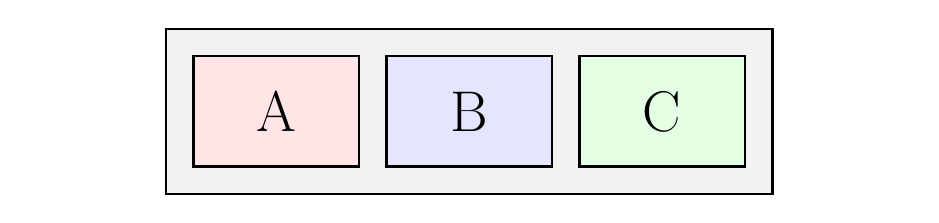
\begin{tikzpicture}[scale=0.07,rotate=0]
	
	%Background
	\draw[draw=white, fill=white] (0,0) rectangle (160,30);
		
	%Frame
	\draw[thick, draw=black, fill=gray!10] (25,0) rectangle (135,30);

	%Segments
	%A
	\draw[thick, draw=black, fill=red!10] (30,5) rectangle (60,25);
	\node at (45,15) {\huge A};

	%B
	\draw[thick, draw=black, fill=blue!10] (65,5) rectangle (95,25);
	\node at (80,15) {\huge B};
	
	%C
	\draw[thick, draw=black, fill=green!10] (100,5) rectangle (130,25);
	\node at (115,15) {\huge C};
	

	
\end{tikzpicture}
\end{document}}
	\caption{Protokoll för överföring av styrkommandon\label{styrdata}}	
\end{figure}

Respektive segment motsvarar följande: 
\begin{itemize}
	\item A (1 byte) - Kommunikations-ID, se tabell \ref{kommunikationstab}.
	\item B (1 byte) - Definierar vilket kommando som skickas, se tabell \ref{styrtab}.
	\item C (1 byte) - Hastighet (om manuellt läge), sträcka/vinkel (om autonomt läge)(tillåtna värden: 0-245).
\end{itemize}

\subsubsection{Kommunikationsprotokoll - kartinformation}
Huvudmodulen kommer för varje ny kartmodul skicka data till datormodulen som ritar upp den nya informationen grafiskt. 

Varje korsning kommer att representeras som en nod och vägarna däremellan som bågar. För att så enkelt som möjligt överföra denna information från huvudmodulen till datormodulen kommer varje nod att representeras enligt protokollet nedan:

 \begin{figure}[H]
\centering
\noindent\resizebox{.8\linewidth}{!}{
	\documentclass[crop,tikz]{standalone}
\usepackage{tikz}
\usetikzlibrary{calc}
\usetikzlibrary{positioning}
\begin{document}
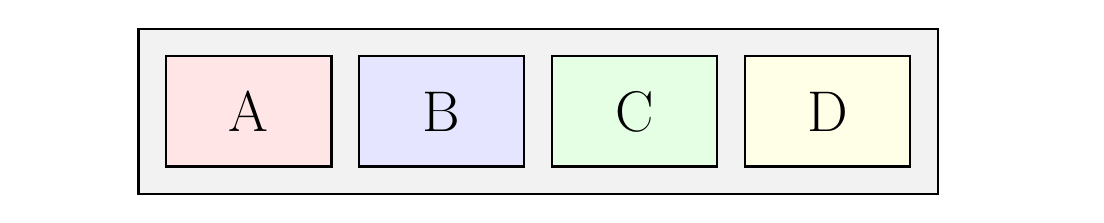
\begin{tikzpicture}[scale=0.07,rotate=0]
		
	%Background
	\draw[draw=white, fill=white] (0,0) rectangle (190,30);	
		
	%Frame
	\draw[thick, draw=black, fill=gray!10] (20,0) rectangle (165,30);

	%Segments
	%A
	\draw[thick, draw=black, fill=red!10] (25,5) rectangle (55,25);
	\node at (40,15) {\huge A};

	%B
	\draw[thick, draw=black, fill=blue!10] (60,5) rectangle (90,25);
	\node at (75,15) {\huge B};
	
	%C
	\draw[thick, draw=black, fill=green!10] (95,5) rectangle (125,25);
	\node at (110,15) {\huge C};
	
	%D
	\draw[thick, draw=black, fill=yellow!10] (130,5) rectangle (160,25);
	\node at (145,15) {\huge D};
	
\end{tikzpicture}
\end{document}}
	\caption{Protokoll för överföring av kartdata \label{kartdata}}	
\end{figure} 

Respektive segment motsvarar följande: 
\begin{itemize}
	\item A (1 byte) - Kommunikations-ID.
	\item B (1 byte) - Motsvarar nodens x-koordinat (tillåtna värden: 0-15).
	\item C (1 byte) - Motsvarar nodens y-koordinat (tillåtna värden: 0-15).
	\item D (1 byte) - Representerar väggar kring noden (11 = vägg, 00 = ingen vägg) i nordlig, västlig, sydlig och östlig riktning (b0-1 = N, b2-3 = W, b4-5 = S, b6-7 = E).
\end{itemize}

\subsubsection{Kommunikationsprotokoll - sensordata}
Sensordata skickas enligt följande protokoll:

 \begin{figure}[H]
\centering
\noindent\resizebox{.8\linewidth}{!}{
	\documentclass[crop,tikz]{standalone}
\usepackage{tikz}
\usetikzlibrary{calc}
\usetikzlibrary{positioning}
\begin{document}
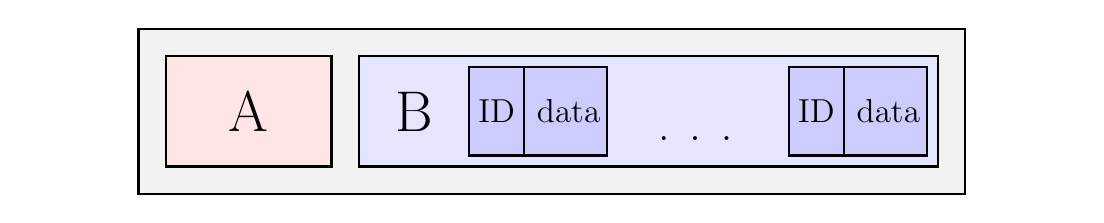
\begin{tikzpicture}[scale=0.07,rotate=0]
	
	%Background
	\draw[draw=white, fill=white] (0,0) rectangle (190,30);
		
	%Frame
	\draw[thick, draw=black, fill=gray!10] (20,0) rectangle (170,30);

	%Segments
	%A
	\draw[thick, draw=black, fill=red!10] (25,5) rectangle (55,25);
	\node at (40,15) {\huge A};

	%B
	\draw[thick, draw=black, fill=blue!10] (60,5) rectangle (165,25);
	\node at (70,15) {\huge B};
	
	%B1
	\draw[thick, draw=black, fill=blue!20] (80,7) rectangle (90,23);
	\draw[thick, draw=black, fill=blue!20] (90,7) rectangle (105,23);
	\node at (85,15) {\large ID};
	\node at (98,15) {\large data};
	
	\node at (121,10) {\LARGE . . .};
	
	%Bn
	\draw[thick, draw=black, fill=blue!20] (148,7) rectangle (163,23);
	\draw[thick, draw=black, fill=blue!20] (138,7) rectangle (148,23);
	\node at (143,15) {\large ID};
	\node at (156,15) {\large data};
	
\end{tikzpicture}
\end{document}}
	\caption{Protokoll för överföring av sensordata\label{sensordata}}	
\end{figure} 

Respektive segment motsvarar följande: 
\begin{itemize}
	\item A - Kommunikations-ID
	\item B - Sensordatapaket
	\begin{itemize}
	\item ID (1 byte) - identifierar sensorn, se tabell \ref{sensortab}.
	\item Data (1 byte) - sensorns värde (tillåtna värden: 0-245).
	\end{itemize}
\end{itemize}

\subsubsection{Kommunikationsprotokoll - styrinställningar}
Följande protokoll används för att skicka styrinställningar (gäller både för datormodul $\rightarrow$ huvudmodul och huvudmodul $\rightarrow$ styrmodul):

\begin{figure}[htbp]
\centering
\noindent\resizebox{.8\linewidth}{!}{
	\documentclass[crop,tikz]{standalone}
\usepackage{tikz}
\usetikzlibrary{calc}
\usetikzlibrary{positioning}
\begin{document}
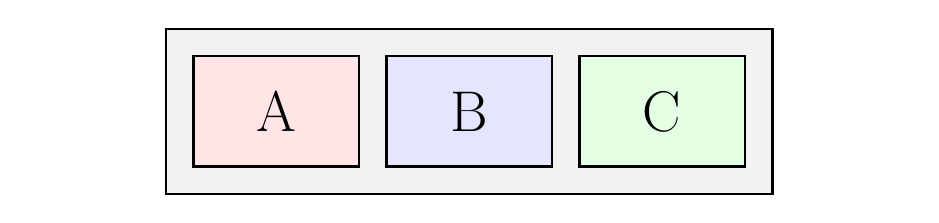
\begin{tikzpicture}[scale=0.07,rotate=0]
	
	%Background
	\draw[draw=white, fill=white] (0,0) rectangle (160,30);
		
	%Frame
	\draw[thick, draw=black, fill=gray!10] (25,0) rectangle (135,30);

	%Segments
	%A
	\draw[thick, draw=black, fill=red!10] (30,5) rectangle (60,25);
	\node at (45,15) {\huge A};

	%B
	\draw[thick, draw=black, fill=blue!10] (65,5) rectangle (95,25);
	\node at (80,15) {\huge B};
	
	%C
	\draw[thick, draw=black, fill=green!10] (100,5) rectangle (130,25);
	\node at (115,15) {\huge C};
	

	
\end{tikzpicture}
\end{document}}
	\caption{Protokoll för överföring av styrkommandon\label{styrdata}}	
\end{figure}

Respektive segment motsvarar följande: 
\begin{itemize}
	\item A (1 byte) - Kommunikations-ID, se tabell \ref{kommunikationstab}.
	\item B (1 byte) - Definierar vilken styrinställning som skickas, se tabell \ref{styrinsttab}.
	\item C (4 byte) - 0/1 om av/på. Annars flyttal (C float).
\end{itemize}

\subsection{Tabeller}

\begin{longtable}[l]{| l | l | c |} \hline
\textbf{ID} & \textbf{Sensor} & \textbf{Enhet} \\ \hline 
1 & IR-sensor höger-fram & cm \\ \hline
2 & IR-sensor vänster-fram  & cm \\ \hline
3 & IR-sensor höger-bak  & cm  \\ \hline
4 & IR-sensor vänster-bak  &  cm \\ \hline
5 & Lasersensor & cm  \\ \hline
6 & Rotation kring z-axeln & rad/s \\ \hline
7 & IR-sensor för mål & cm \\ \hline
\caption{Tabell över sensorerna}\label{sensortab}
\end{longtable}

\begin{longtable}[l]{| l | l |} \hline
\textbf{ID} & \textbf{Styrkommando} \\ \hline 
1 & Kör fram \\ \hline
2 & Kör bak \\ \hline
3 & Rotera åt höger \\ \hline
4 & Rotera åt vänster \\ \hline
5 & Fram och höger \\ \hline
6 & Fram och vänster \\ \hline
7 & Bak och höger \\ \hline
8 & Bak och vänster \\ \hline
9 & Gripklo öppna/stäng \\ \hline

\caption{Tabell över styrkommandon}\label{styrtab}
\end{longtable}

\begin{longtable}[l]{| l | l |} \hline
\textbf{ID} & \textbf{Styrinställning} \\ \hline 
1 & Reglering av/på \\ \hline
2 & P-värde \\ \hline
3 & D-värde \\ \hline
4 & K-värde \\ \hline

\caption{Tabell över styrinställningar}\label{styrinsttab}
\end{longtable}

\section{Slutsatser}
\textit{Vilka förbättringar skulle kunna göras?}

\pagebreak
\addcontentsline{toc}{section}{Referenser}
\bibliographystyle{ieeetr}
\bibliography{references}

\pagebreak


\appendix

\end{flushleft}

\end{document}
